\begin{figure*}
    \centering
    \begin{subfigure}{\textwidth}
        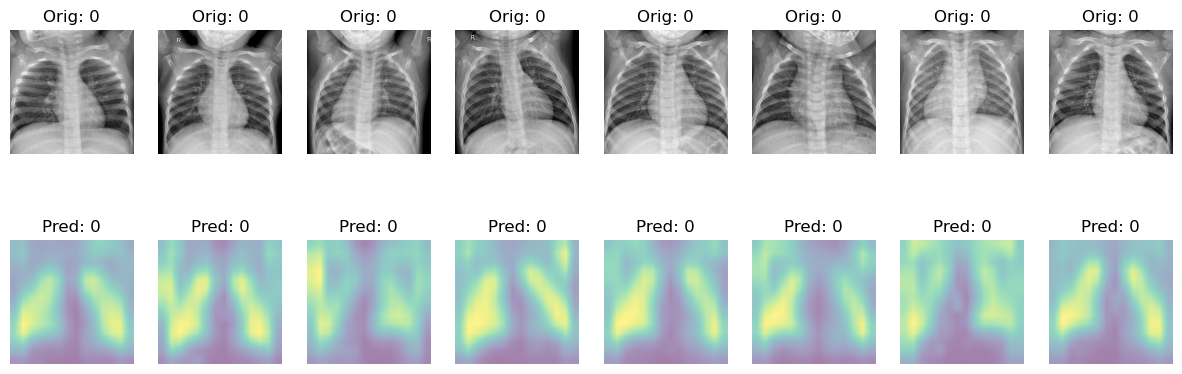
\includegraphics[width=1\textwidth]{images/gc_train.png}
    \end{subfigure}
    \centering
    \begin{subfigure}{\textwidth}
        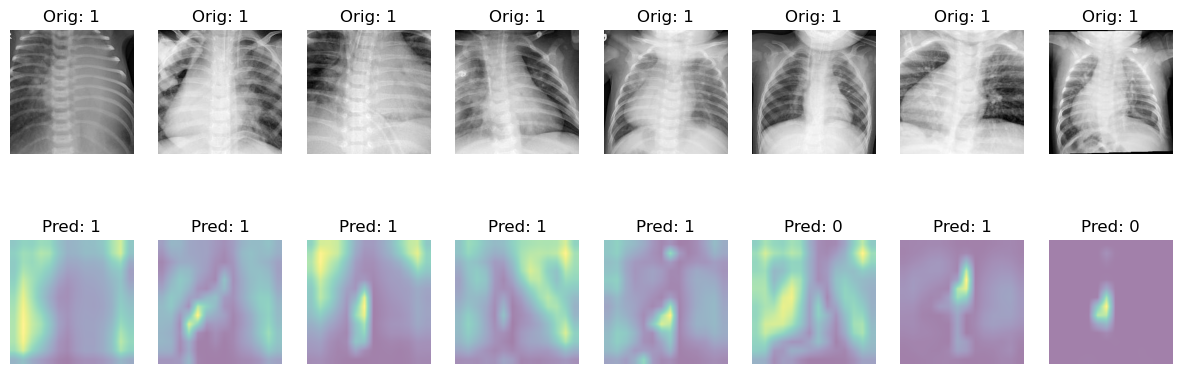
\includegraphics[width=1\textwidth]{images/gc_train_P.png}
    \end{subfigure}
    \caption{Training images to which Grad-CAM was applied. Upper two rows are from healthy patients, bottom two rows from patients with pneumonia. The 1st and 3rd row contain the input image, the 2nd and 4th row contain the overlay produced by Grad-CAM. Yellow signifies the highest attribution, purple the lowest attribution.}
    \label{fig:gc_train}
\end{figure*}

\section{Grad-CAM}

Grad-CAM is a method that highlights parts of an image based on the contribution of the respective neurons for class prediction. For this, Grad-CAM uses gradients between the last convolutional layer and the decisions of the output layer.
For our implementation, we modify the code from \cite{gradcam}.

\subsection*{A. Visualization}
If we look at the results on the training dataset in Figure \ref{fig:gc_train}, the pattern in healthy patients is very consistent, with the main focus on the lungs, and little focus on everything below the diaphragm. In addition, the hilum of the lungs (where the airways 'enter' the lungs) is also represented well, but this is partially 'masked out' due to the many overlapping structures nearby, such as the heart and the vertebra.

The model does not explain finer details due to the fact that Grad-CAM only produces a coarse localization map.

For sick patients, both global and local importance can be seen, the global focus on the lungs similar to healthy patients (albeit sometimes absent).

\begin{figure}
    \centering
    \begin{subfigure}{\columnwidth}
        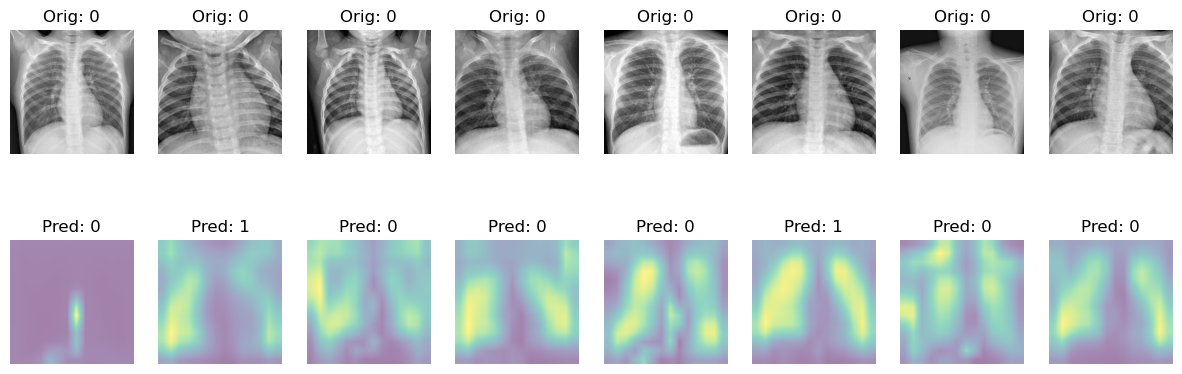
\includegraphics[width=1\textwidth]{images/gc_test.png}
    \end{subfigure}
    \centering
    \begin{subfigure}{\columnwidth}
        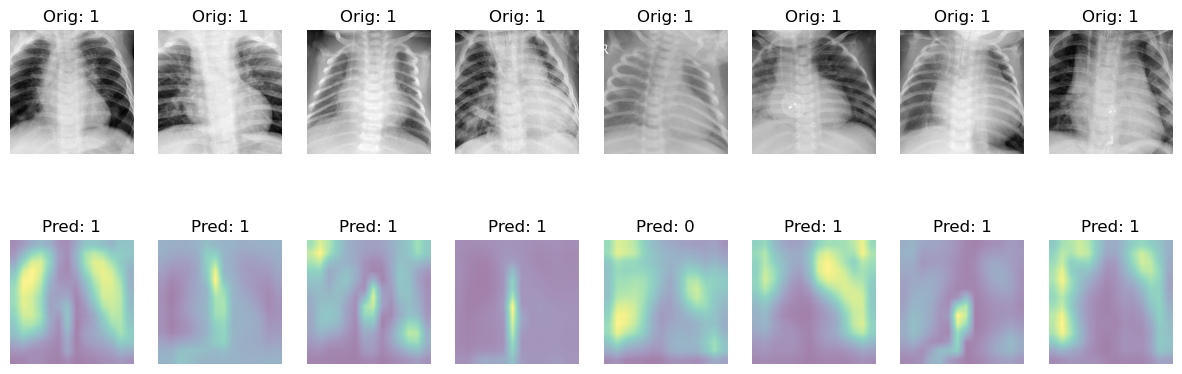
\includegraphics[width=1\textwidth]{images/gc_test_P.png}
    \end{subfigure}
    \caption{Test images to which Grad-CAM was applied. Upper two rows are from healthy patients, bottom two rows from patients with pneumonia. The 1st and 3rd row contain the input image, the 2nd and 4th row contain the overlay produced by Grad-CAM. Yellow signifies the highest attribution, purple the lowest attribution.}
    \label{fig:gc_test}
\end{figure}

The local importance at the vertebra seems a bit odd, although there might be some enlarged lymph nodes there. An alternative hypothesis is that the patient might have a feeding tube in place, which would make sense, as sick children often refuse to eat food. An additional contributing factor might be that the images from the healthy patients are more similar to one another, both in positioning of the child andin terms of radiological findings, while sick children with many different radiological findings are more difficult to keep in a fixed position during imaging.

All in all, we can conclude that the model knows that the lungs are the most important part of the X-ray image that contributes to the final prediction, but is still sometimes confused by the intra-class differences of sick patients.

All previously mentioned patterns can also be seen in images in the test set in Figure \ref{fig:gc_test}.